\documentclass[border=6pt]{standalone}
\usepackage{tikz}
\usepackage{pgfplots}
\pgfplotsset{compat=1.16}
\usepackage{amsmath}
\begin{document}
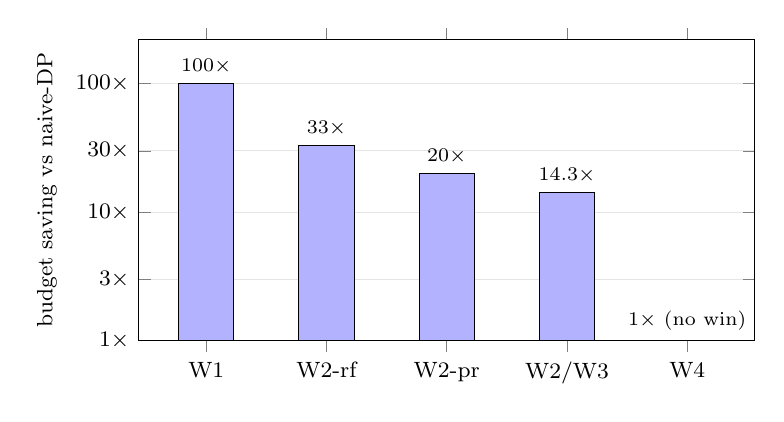
\begin{tikzpicture}
\begin{axis}[
  width=9.4cm, height=5.4cm,
  ybar, bar width=20pt,
  ymode=log, log origin=infty,
  ymin=1, ymax=220,
  ytick={1,3,10,30,100},
  yticklabels={$1\times$,$3\times$,$10\times$,$30\times$,$100\times$},
  ylabel={budget saving vs naive-DP},
  symbolic x coords={W1,W2{-}rf,W2{-}pr,W2/W3,W4},
  xtick=data,
  nodes near coords, point meta=explicit symbolic,
  nodes near coords style={font=\scriptsize, anchor=south},
  tick label style={font=\footnotesize}, label style={font=\footnotesize},
  enlarge x limits=0.14,
  ymajorgrids, grid style={gray!20},
]
\addplot[fill=blue!30, draw=black] coordinates {
  (W1,100)   [$100\times$]
  (W2{-}rf,33) [$33\times$]
  (W2{-}pr,20) [$20\times$]
  (W2/W3,14.3) [$14.3\times$]
  (W4,1)     [$1\times$ (no win)]
};
\end{axis}
\end{tikzpicture}
\end{document}
